\documentclass[conference]{IEEEtran}
\IEEEoverridecommandlockouts

\usepackage{cite}
\usepackage{amsmath,amssymb,amsfonts}
\usepackage{graphicx}
\usepackage{textcomp}
\usepackage{xcolor}
\usepackage{booktabs}
\usepackage{array}
\usepackage{url}
\usepackage{tikz}

\begin{document}

\title{Gate-Reconstruction Learning for Metasurface-Inspired ISRJ Parameter Estimation}

\author{
\IEEEauthorblockN{Author One, Author Two, Author Three}
\IEEEauthorblockA{
Affiliation placeholder \\
City, Country \\
email placeholder
}
}

\maketitle

\begin{abstract}
Classical intermittent sampling repeater jamming (ISRJ) parameter estimation usually assumes ideal rectangular gating. That assumption becomes weak when the deceptive waveform keeps a finite low-scattering state instead of switching fully off. This paper addresses that case with a gate-reconstruction learning framework for estimating slice width, sampling interval, and low-state coefficient from raw IQ data. The model predicts the three parameters and reconstructs the periodic gate profile at the same time, so the estimation process stays tied to the waveform structure that produces the deceptive echo. The method reaches an overall accuracy of $83.61\%$, and its accuracy rises to $95.62\%$ when JNR is above $0$ dB. These findings suggest that reconstructing the gate profile helps the model estimate the three parameters more reliably, while low-JNR robustness remains the main weakness.
\end{abstract}

\begin{IEEEkeywords}
radar countermeasure, interrupted sampling, metasurface-inspired deception, parameter estimation, transformer network
\end{IEEEkeywords}

\section{Introduction}
Intermittent sampling repeater jamming (ISRJ) is an important form of coherent repeater jamming. The jammer intercepts the radar signal, samples it in short slices, and retransmits the samples after delay \cite{wang2007}. This sampling-and-retransmission process can generate multiple false targets while avoiding full-pulse storage \cite{feng2017}. The timing law is therefore central to both jamming analysis and countermeasure design. For this reason, classical ISRJ studies have focused mainly on slice width, sampling interval, and the resulting false-target structure \cite{wang2021admm,wei2018}.

Deep learning has recently been introduced into radar jamming analysis and parameter inference. Wang \emph{et al.} \cite{wang2026ast} estimate ISRJ parameters through an end-to-end pipeline that combines separation and measurement. Lu \emph{et al.} \cite{lu2025rs} also couple recognition and parameter estimation in a detection-style framework. These studies show that data-driven models can reduce the dependence on handcrafted processing. However, they are still built around conventional ISRJ waveform assumptions.

In metasurface-inspired ISRJ, the returned waveform is governed by switching between high- and low-scattering states. Sun \emph{et al.} \cite{sun2024tmtt} describe how periodic switching between reflection states can manipulate radar echoes. Ding \emph{et al.} \cite{ding2025tmtt} further show that time-modulated metasurfaces can be used in radar jamming applications. Cai and Li \cite{cai2024} extend this picture by using simultaneous phase and amplitude coding to realize multi-frequency electromagnetic modulation, which supports a two-state view with a nonzero low-scattering level. Existing ISRJ parameter-estimation studies do not directly address this case, where the waveform departs from ideal rectangular gating but still retains periodic structure.

This paper studies parameter estimation for metasurface-inspired ISRJ with a normalized high-scattering state and a nonzero low-scattering state. The goal is to estimate slice width, sampling interval, and low-state coefficient from raw IQ observations. These parameters are all governed by the same periodic gate pattern. A direct three-output regressor does not enforce that structure explicitly. This paper therefore uses a reconstruction-guided estimator that predicts the three parameters while also recovering the gate profile. In this way, parameter estimation remains tied to the waveform structure that produces the jamming signal. Its main contributions are:
\begin{enumerate}
\item A reconstruction-guided estimator that jointly predicts slice width, sampling interval, and low-state coefficient while recovering the underlying periodic modulation waveform.
\item Strong results on the current benchmark, including high accuracy when JNR is above $0$ dB.
\end{enumerate}

The remainder of the paper defines the signal model, presents the proposed method, and reports the experimental results.

\section{Signal Model and Problem Formulation}
In this paper, metasurface-inspired ISRJ is described by periodic switching between a high-scattering state and a low-scattering state. This choice bridges the gap between idealized ISRJ gating and metasurface-inspired two-state modulation. A linear-frequency-modulated waveform is used as the base signal. The target delay and the deceptive delay are denoted by $\tau_t$ and $\tau_j$, respectively.

After normalizing the high-scattering state to one and denoting the low-state coefficient by $x_{\text{low}} \in [0, 0.5]$, the modulation waveform is written as
\begin{equation}
\begin{aligned}
p(t)={}&\left(1-x_{\text{low}}\right)\operatorname{rect}\!\left(\frac{t-\tau_j}{T_l}\right) \otimes \\
&\sum_{k=-\infty}^{+\infty}\delta\left(t-\tau_j-kT_s\right) + x_{\text{low}},
\end{aligned}
\end{equation}
where $\operatorname{rect}(\cdot)$ denotes the rectangular pulse, $\otimes$ denotes convolution, $T_l$ is the slice width, and $T_s$ is the sampling interval. In this form, the effective scattering coefficient switches periodically between a normalized high-scattering state of $1$ and a low-scattering state of $x_{\text{low}}$.

\begin{figure}[t]
\centering
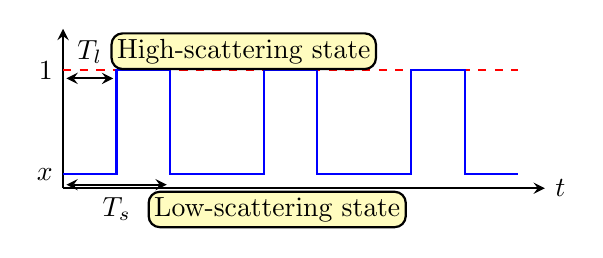
\begin{tikzpicture}[x=0.85cm,y=1.5cm,>=stealth,thick]
  \draw[->] (0,0) -- (7.2,0) node[right] {$t$};
  \draw[->] (0,0) -- (0,1.35);
  \node[left] at (0,1) {$1$};
  \node[left] at (0,0.12) {$x$};
  \draw[red,dashed] (0,1) -- (6.8,1);
  \draw[blue] (0,0.12) -- (0.8,0.12) -- (0.8,1) -- (1.6,1) -- (1.6,0.12)
              -- (3.0,0.12) -- (3.0,1) -- (3.8,1) -- (3.8,0.12)
              -- (5.2,0.12) -- (5.2,1) -- (6.0,1) -- (6.0,0.12) -- (6.8,0.12);
  \draw[<->] (0.05,0.93) -- (0.75,0.93);
  \node[above] at (0.4,0.97) {$T_l$};
  \draw[<->] (0.05,0.03) -- (1.55,0.03);
  \node[below] at (0.8,0.01) {$T_s$};
  \node[draw, fill=yellow!25, rounded corners, inner sep=2pt] at (2.7,1.16) {High-scattering state};
  \node[draw, fill=yellow!25, rounded corners, inner sep=2pt] at (3.2,-0.18) {Low-scattering state};
\end{tikzpicture}
\caption{Time modulation model with alternating high- and low-scattering states.}
\label{fig:time_modulation_model}
\end{figure}

The metasurface-inspired ISRJ signal is then expressed as
\begin{equation}
r_j(t)=p(t)\,s(t-\tau_j),
\end{equation}
and the received signal becomes
\begin{equation}
r(t)=s(t-\tau_t)+r_j(t)+n(t),
\end{equation}
where $n(t)$ is complex Gaussian noise. The parameter-estimation target is the vector
\begin{equation}
\mathbf{y}=[T_l,\; T_s,\; x_{\text{low}}]^\top.
\end{equation}
For consistency with classical ISRJ terminology, the rest of the paper refers to $T_l$ as slice width and to $T_s$ as sampling interval.

Two derived quantities help interpret estimation difficulty. The first is the duty ratio $\eta=T_l/T_s$, which gives the fraction of each period spent in the high-scattering state. The second is the timing gap $T_s-T_l$, which measures the separation between adjacent high-scattering segments. Together, they indicate when the waveform approaches a near-continuous retransmission regime. Both quantities reappear later in the confidence analysis because they mark physically meaningful hard operating regions.

\section{Proposed Method}
Given the target vector in Section III, the proposed method estimates slice width, sampling interval, and low-state coefficient directly from raw IQ observations. The main design choice is to reconstruct the periodic gate while predicting the three parameters. Gate reconstruction is not used here as a visualization byproduct. It keeps the estimator tied to the waveform structure that generates the target variables. This makes the method a better match to the signal model than unconstrained scalar regression.

\subsection{Input Representation}
The estimator uses a two-channel IQ input so the representation stays close to the received waveform. The real and imaginary parts are normalized with a dataset-level scale and stacked as a $2 \times N$ tensor. This choice matches the currently trained \texttt{gate\_reconstruction} model and avoids adding handcrafted side features that are not used in the checked training recipe.

\subsection{Gate-Reconstruction Estimator}
The estimator follows a shared-encoder, coupled-decoder design. A one-dimensional convolutional tokenizer first extracts local waveform structure. A strided patch-embedding layer then converts the sequence into latent tokens. These tokens pass through a shared transformer encoder and are summarized into a compact global representation for downstream prediction. The shared encoder is used to preserve the periodic jammer pattern before the model commits to any single output branch.

The encoded summary then feeds three coupled prediction paths:
\begin{enumerate}
\item a timing head that predicts normalized sampling interval,
\item a coefficient head that predicts normalized low-state coefficient,
\item a gate head that reconstructs a discretized periodic gate profile.
\end{enumerate}

The timing embedding is reused when decoding the low-state coefficient and gate profile, so the model does not treat the three targets as unrelated scalars. In practice, the network first learns a representation of periodic modulation. It then decodes the physical parameters from that shared structure. This is the main difference from a direct three-output regressor.

\subsection{Training Objective and Physical Decoding}
Let $\hat{\mathbf{y}}$ denote the decoded physical predictions, and let $\hat{\mathbf{g}}$ denote the reconstructed full-length jammer mask. The training objective combines weighted parameter regression, mask reconstruction, and temporal smoothing:
\begin{equation}
\mathcal{L}=\mathcal{L}_{\text{reg}} + \lambda_r \mathcal{L}_{\text{mask}} + \lambda_{tv} \mathcal{L}_{tv},
\end{equation}
where $\mathcal{L}_{\text{reg}}$ is a weighted smooth-$L_1$ loss over $T_l$, $T_s$, and $x_{\text{low}}$, $\mathcal{L}_{\text{mask}}$ compares the reconstructed and true jammer masks, and $\mathcal{L}_{tv}$ penalizes excessive variation across adjacent bins of the decoded gate period. In the checked configuration, the parameter loss weights emphasize slice-width error most strongly, followed by low-state-coefficient error and then sampling-interval error. This weighting comes directly from the checked training recipe.

After training, normalized outputs are mapped back to physical units using the same scaler ranges that define the synthetic dataset. The decoder also enforces the dataset's minimum interval-gap constraint, so predicted timing values remain inside a physically meaningful region. The final output is still the physical parameter tuple of Section III, but it is obtained through an intermediate representation that resembles a realizable periodic gate profile.

\subsection{Auxiliary Confidence Analysis}
In addition to point estimation, the repository defines a lightweight confidence score derived from physically meaningful margins: duty ratio, low-state-coefficient risk, timing-gap margin, and boundary margin. These terms are combined into a scalar risk score and converted into a confidence score in $[0,1]$. This module is not a second primary contribution. It serves as an auxiliary analysis tool to test whether the estimator can flag geometrically difficult operating points in addition to returning parameter predictions.

\section{Experimental Results}
\subsection{Experimental Setup}
The experiments test whether the proposed estimator can recover the parameter tuple of Section III in the synthetic single-component setting used in this paper. The checked dataset configuration exports $6200$ training samples, $775$ validation samples, and $775$ held-out test samples. The JNR sweep is discrete and balanced across integer values from $-10$ dB to $20$ dB. Duty-cycle coverage is stabilized through four bins, so the model is not trained on a narrow subset of timing regimes.

The checked training configuration uses batch size $16$, learning rate $3\times 10^{-4}$, weight decay $10^{-4}$, and $64$ end-to-end epochs. The selected architecture uses two input channels, hidden width $128$, four shared transformer layers, and a gate decoder with $128$ bins. Unless otherwise stated, all quantitative results are reported on the held-out test split of this configuration.

\subsection{Evaluation Metrics}
Both mean absolute error (MAE) and accuracy are reported so that the evaluation reflects both average deviation and operational tolerances. Let $N_{\text{test}}$ denote the number of test samples. Let $\hat{T}_{l,i}$, $\hat{T}_{s,i}$, and $\hat{x}_{\text{low},i}$ denote the predicted parameters of sample $i$, and let $T_{l,i}$, $T_{s,i}$, and $x_{\text{low},i}$ denote the corresponding ground-truth values. The three per-parameter accuracy metrics are defined as
\begin{equation}
A_{T_l}=\frac{1}{N_{\text{test}}}\sum_{i=1}^{N_{\text{test}}}\mathbb{I}\!\left(\left|\hat{T}_{l,i}-T_{l,i}\right|\le 0.15~\mu\text{s}\right)\times 100\%,
\end{equation}
\begin{equation}
A_{T_s}=\frac{1}{N_{\text{test}}}\sum_{i=1}^{N_{\text{test}}}\mathbb{I}\!\left(\left|\hat{T}_{s,i}-T_{s,i}\right|\le 0.25~\mu\text{s}\right)\times 100\%,
\end{equation}
\begin{equation}
A_{x}=\frac{1}{N_{\text{test}}}\sum_{i=1}^{N_{\text{test}}}\mathbb{I}\!\left(\left|\hat{x}_{\text{low},i}-x_{\text{low},i}\right|\le 0.05\right)\times 100\%,
\end{equation}
where $\mathbb{I}(\cdot)$ is the indicator function. For compactness, let $\mathcal{E}_i$ denote the event that all three parameter errors of sample $i$ satisfy their respective tolerances. Total accuracy is then defined as
\begin{equation}
A_{\text{total}}=\frac{1}{N_{\text{test}}}\sum_{i=1}^{N_{\text{test}}}\mathbb{I}(\mathcal{E}_i)\times 100\%.
\end{equation}

\subsection{Main Results}
The first experiment tests whether the gate-reconstruction estimator can recover all three target parameters on the held-out test split. Table~\ref{tab:overall_results} shows that the answer is yes in most cases. The model reaches an $83.61\%$ total accuracy, which means all three parameters fall within their prescribed tolerances for the majority of test samples.

The per-parameter results show a clear pattern. Slice width and sampling interval are easier to recover, with mean absolute errors of $0.0573~\mu$s and $0.0994~\mu$s and accuracies above $94\%$. The low-state coefficient is harder, with a mean absolute error of $0.0270$ and an accuracy of $87.48\%$. This gap is reasonable. Periodic timing structure is reflected more directly in the received waveform, while the low-state coefficient is more sensitive to noise and local gate-reconstruction error. Overall, the main weakness of the current model is coefficient-level estimation, not timing recovery.

The same conclusion remains stable across random initializations. Over five independent training runs, the mean total accuracy is $81.63\%$ with a standard deviation of $1.38$ percentage points. The corresponding low-JNR total accuracy is $53.20\%$ with a standard deviation of $2.30$ percentage points. These numbers show that the method does not depend on a single favorable seed. Instead, it produces a relatively narrow performance band across runs. This supports the reproducibility of the current training setup.

\begin{table}[t]
\centering
\caption{Overall parameter recovery results on the held-out test split. Total accuracy requires all three parameters to satisfy their respective tolerances.}
\label{tab:overall_results}
\begin{tabular}{lcc}
\toprule
Parameter & MAE & Accuracy (\%) \\
\midrule
Slice width ($\mu$s) & 0.0573 & 94.45 \\
Sampling interval ($\mu$s) & 0.0994 & 96.52 \\
Low-state coefficient & 0.0270 & 87.48 \\
Total & -- & 83.61 \\
\bottomrule
\end{tabular}
\end{table}

\subsection{Robustness Across JNR Regimes}
To locate the remaining errors, performance is further broken down by JNR regime. Table~\ref{tab:jnr_slices} shows that most of the degradation is concentrated in the lowest-JNR range. In $[-10,0)$~dB, total accuracy drops to $58.40\%$. It then rises quickly to $90.67\%$, $96.67\%$, and $98.22\%$ in the $[0,6)$, $[6,12)$, and $[12,20]$~dB ranges, respectively.

This result matters because it clarifies what is limiting the model. The method already recovers the interrupted-sampling structure reliably in moderate and high JNR conditions. The overall error budget is instead dominated by a relatively small set of hard low-JNR cases. A finer-grained inspection of the pointwise JNR slices shows the same pattern: at $-10$~dB, total accuracy falls to $8\%$. At that point, both gate shape and low-state coefficient become difficult to infer because the jammer signature is strongly masked by noise. The main future target is therefore low-JNR robustness, not a redesign of the overall modeling framework.

\begin{table}[t]
\centering
\caption{Parameter recovery across JNR regimes on the test split. The main degradation is concentrated in the lowest-JNR range.}
\label{tab:jnr_slices}
\resizebox{\columnwidth}{!}{%
\begin{tabular}{lcccc}
\toprule
JNR range (dB) & Count & Slice-width MAE & Sampling-interval MAE & Total accuracy (\%) \\
\midrule
$[-10,0)$ & 250 & 0.1113 & 0.1968 & 58.40\% \\
$[0,6)$   & 150 & 0.0327 & 0.0569 & 90.67\% \\
$[6,12)$  & 150 & 0.0284 & 0.0502 & 96.67\% \\
$[12,20]$ & 225 & 0.0329 & 0.0524 & 98.22\% \\
\bottomrule
\end{tabular}
}
\end{table}

\begin{table}[t]
\centering
\caption{Reproducibility across five random seeds. Results are reported as mean, standard deviation, minimum, and maximum.}
\label{tab:stability}
\resizebox{\columnwidth}{!}{%
\begin{tabular}{lcccc}
\toprule
Metric & Mean & Std & Min & Max \\
\midrule
Total accuracy (\%) & 81.63 & 1.38 & 79.48 & 82.97 \\
Low-JNR total accuracy (\%) & 53.20 & 2.30 & 51.20 & 56.80 \\
Slice-width accuracy (\%) & 92.70 & 0.89 & 91.35 & 93.55 \\
Sampling-interval accuracy (\%) & 95.17 & 0.64 & 94.45 & 96.00 \\
Low-state-coefficient accuracy (\%) & 86.55 & 1.30 & 84.52 & 87.87 \\
\bottomrule
\end{tabular}
}
\end{table}

\section{Conclusion}
This paper presented a gate-reconstruction learning framework for parameter estimation under a metasurface-inspired interrupted-sampling deception model with a nonzero low-state coefficient. The main idea is to couple parameter decoding with periodic gate recovery instead of treating the task as three independent scalar regressions.

On the current synthetic benchmark, the method reaches an $83.61\%$ total accuracy on the held-out test split. Performance is already near-saturated in moderate- and high-JNR regimes. The results also remain stable across random initializations. The main unresolved weakness is robustness in extremely low JNR conditions.

These findings support the central claim of the paper: under the considered two-state ISRJ model, reconstructing the gate profile helps the model estimate slice width, sampling interval, and low-state coefficient more reliably. The present study is limited to a simulation-based single-component setting with a narrow jammer family and one heuristic baseline. The claims should therefore be read within that scope. Future work should strengthen low-JNR robustness, extend the benchmark to broader jammer families, and validate the framework beyond the current single-component synthetic setting.


\section*{Acknowledgment}
Funding and project acknowledgments should be inserted here after the author block is finalized.

\begin{thebibliography}{00}
\bibitem{wang2007} X. Wang, J. Liu, W. Zhang, Q. Fu, Z. Liu, and X. Xie, ``Mathematic principles of interrupted-sampling repeater jamming (ISRJ),'' \emph{Science in China Series F: Information Sciences}, vol. 50, no. 1, pp. 113--123, Feb. 2007.
\bibitem{feng2017} D. Feng, L. Xu, X. Pan, and X. Wang, ``Jamming wideband radar using interrupted-sampling repeater,'' \emph{IEEE Transactions on Aerospace and Electronic Systems}, vol. 53, no. 3, pp. 1341--1354, Jun. 2017.
\bibitem{wang2021admm} C. Wang, W. Hu, Z. Geng, J. Zhang, and D. Zhu, ``Parameter estimation for interrupted sampling repeater jamming based on ADMM,'' \emph{Sensors}, vol. 21, no. 24, Art. no. 8277, Dec. 2021.
\bibitem{wei2018} Z. Wei, Z. Liu, B. Peng, and R. Shen, ``ECCM scheme against interrupted sampling repeater jammer based on parameter-adjusted waveform design,'' \emph{Sensors}, vol. 18, no. 4, Art. no. 1141, Apr. 2018.
\bibitem{wang2026ast} G. Wang, Q. Lv, L. Liu, Y. Wu, Y. Quan, R. Yang, and B. Bie, ``An end-to-end deep learning framework for separation and parameter measurement of composite intermittent sampling repeater jamming,'' \emph{Aerospace Science and Technology}, vol. 168, Art. no. 111218, 2026.
\bibitem{lu2025rs} J. Lu, Y. Guo, W. Feng, X. Hu, J. Gong, and Y. Zhang, ``Intelligent recognition and parameter estimation of radar active jamming based on oriented object detection,'' \emph{Remote Sensing}, vol. 17, no. 15, Art. no. 2646, Jul. 2025.
\bibitem{sun2024tmtt} G. Sun, J. Wang, S. Xing, D. Huang, D. Feng, and X. Wang, ``A flexible conformal multifunctional time-modulated metasurface for radar characteristics manipulation,'' \emph{IEEE Transactions on Microwave Theory and Techniques}, vol. 72, no. 7, pp. 4294--4308, Jul. 2024.
\bibitem{ding2025tmtt} C. Ding, H. Mu, H. Mu, Y. Meng, M. Zhao, Y. Zhang, T. Cai, F. Meng, F.-Y. Meng, and J. Wang, ``Time-modulated metasurface-assisted moving target jamming for synthetic aperture radar,'' \emph{IEEE Transactions on Microwave Theory and Techniques}, vol. 73, no. 7, pp. 4191--4203, Jul. 2025.
\bibitem{cai2024} C. Cai and Y. Li, ``Phase and amplitude simultaneously coding metasurface with multi-frequency and multifunctional electromagnetic modulations,'' \emph{Scientific Reports}, vol. 14, Art. no. 20904, Sep. 2024.
\end{thebibliography}

\end{document}
